\chapter{Technology and method}
\lhead{\emph{Technology and method}}

% Hardkoding og logikk for søk etter kontekst
% 

\section{Introduction}
% Var vi limited til å følge matistikk?
In this chapter the technology and methods applied in this project is reasoned. The project was at no point limited to follow Matistikk, but for the sake of simplicity and engineering flexibility tools which both provided good results in short time and if it were to be implemented in Matistikk, a Python solution was preferable.
% TODO Sjekk om jeg ikke prater opp igjen mange ganger


\section{Technology}
The choice of technology was highly influenced by the nature of the project assignment, if the goal was to create a module for an existing Django application, Python was already the obvious choice. Eventually the project drifted in the way of a proof of concept, Python came out even further as the obvious choice. The reason why Python is the obvious choice in this case, is the ability to go from idea to a working prototype in the fastest way possible. In addition to productivity Python has a lot of mature libraries, in the nature of working towards a proof of concept, one would need stable, tested and well documented libraries. We found especially Keras \parencite{chollet_keras_2015} to be a perfect fit for our task, which is a library that makes TensorFlow or some other machine learning library easier to use.\\
\quad
The choice of back end and processing tool was now chosen, Keras backed by TensorFlow is an extremely feature-rich combination. Since the project went in the way of a proof of concept we needed some graphical user interface in which we could collect data, present statistics and so forth. The selection of front end was determined by the project assignment. Since Matistikk is web-based, we found it quite natural to go with some simple HTML, Css, JavaScript and Tornado. Tornado is a simple library to build web servers in Python.

\section{Communication and dataflow}
The foundation was quickly made, that led to an classic client/server approach. Already in the first weeks of the project Keras and deep learning was our focus.% dårlig setning...
The progress made was not only based on our own experimentation. Articles and projects posted was quickly digested and learned from. CROHME gave the project it's desirable data and insight into the assignment. CROHME provided both tools and  sequential data in InkML files, see listing \ref{lst:InkML_ex} for an InkML example file.\\
Even with the new discovered data, the research still continued.  Lu and Mohan \cite{lu_recognition_2015} and Thoma \cite{thoma_-line_2015} inspired the work made in this project. The majority of data at that stage was sequential, a decision was made to use a \gls{WebSocket} to handle front to back end communication. For the sake of simplicity, it was also implemented a way to do this over a simple http post request as an alternative to the WebSocket implementation. Doing it this way created a simple, but solid foundation for the engineers behind Matistikk to do it the way they wanted. \\
After discussion with our project owners, we were drawn to the direction of using a http post request. The test application also does not think about the amount of data it sends per classification request. If the canvas is changed, it still re-sends the entire buffer. This is both to easy re-evaluate the buffer, but in addition this can trigger changes in the segmentation process, which can eventually lead to a different classification.

\section{The recognition system} % TODO vurder om dette er for nært resultat kapittelet. SE MAL
The recognition system consists of both some "hard-coded" logic and the neural network. As stated in chapter 2.1, handwriting recognition includes several steps required to classify correctly. The "hard-coded" logic solves the segmentation issue in an elementary way, but it is quite vulnerable to noisy input. In addition to segmentation we do a whole lot of prepossessing to make sure our actual data flowing from our front end to our back end is roughly the same size format, data type and so forth. % TODO Insert a simple diagram of our system

\section{Artificial Neural Network}
Artificial neural networks in image recognition is often to be found in tutorials. Since the project engineers had no prior experience with artificial neural networks it was necessary to experiment with different types of neural network and data. The MNIST data set consists of handwritten digits which is available in Keras. The amount of thorough tutorials on the MNIST data set inspired the project in new aspects. At that time, there was made a decision to use CNNs to handle the recognition problem. This meant that all the sequential data must be converted into images. \\ This was a decision that turned out to work as desired, it was not a choice that led to success. But the issue was not more focused on handling segmentation and applying different techniques to obtain good accuracy. After some experimentation with CNNs, attempts at getting it done with RNNs was started. The project went into a hard period, where we were battling variable length input and at the same time we felt that our working solution would not improve. % Trenger review..

\section{Classification model}

% The neural network 

\section{Architecture}



\section{Image data}
When deciding on the image format it was clear that the best approach was to resemble an already existing data set in order to obtain more data. Experimenting on the MNIST data made the project engineers explore possibilities to convert our InkML data to grey scale images in the same format as MNIST data. This, of course was no straight forward procedure, after several tries over a couple of weeks it was decided to go forward with generating bitmaps. Generating BMPs was a much simpler task, and luckily we found BMPs that were of handwritten mathematical symbols.

\subsection{Preprocessing}
\begin{figure}[H]
    \centering
    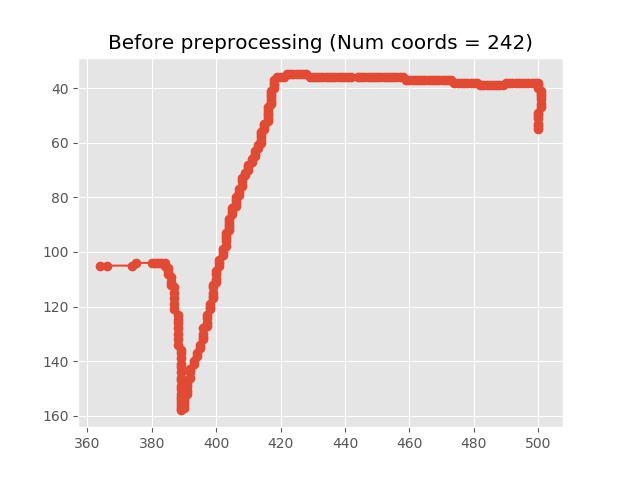
\includegraphics{Assets/Chapter3_Method/sqrt_before_preprocessing.png}
    \caption{A square root which has not been thorough preprocessing.}
    \label{fig:sqrt_not_processed}
\end{figure}

\begin{figure}[H]
    \centering
    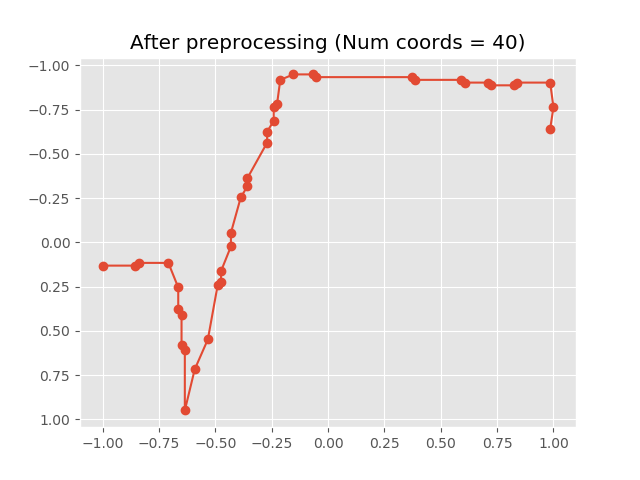
\includegraphics{Assets/Chapter3_Method/sqrt_after_preprocessing.png}
    \caption{A square root which has been through preprocessing.}
    \label{fig:sqrt_processed}
\end{figure}

\begin{figure}[H]
    \centering
    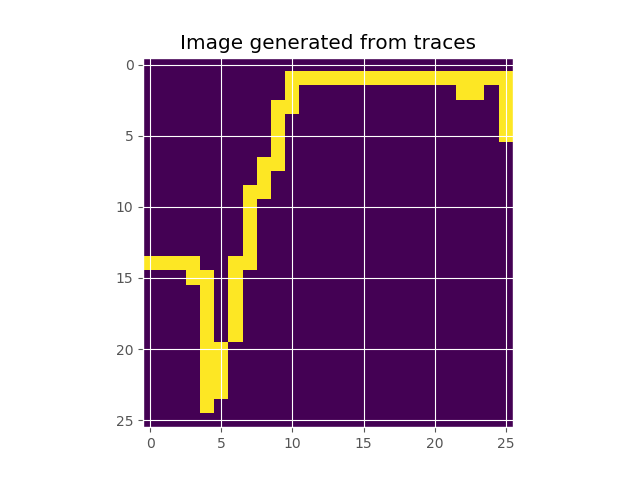
\includegraphics{Assets/Chapter3_Method/sqrt_image.png}
    \caption{The resulting square root from the preprocessing done in previous steps.\\The generated image is 26x26 pixels.}
    \label{fig:sqrt_img}
\end{figure}

\section{Segmentation}
Since the project initially went for a solution with a CNN, we had to separate the system into different tasks. The reason behind this is that the CNN itself, in our solution should solely work on the classification of a symbol. Since our assignment is to handle symbols and expressions, we then need to extract single symbols from multiple symbols or expressions.\\
This specific task was and is the most critical in order to get correct recognition with a CNN. If the segmentation turned out wrong, the classification would be handed bad data which makes a correct classification unlikely.\\ To solve the segmentation issue different approaches was attempted, among those were object localization and detection, with bounding boxes to easily detect symbols which consists of multiple strokes or traces. This idea of object detection was quite good and would have, if successful made the rest quite easy in comparison.\\ The attempts made on object detection was unsuccessful, we were getting results, but they were not proving to be better than solving it with a much simpler algorithm which did not require machine learning in the first place. 


%This decision turned out to be very wise. Eventually new data was discovered, this was from the CROHME competitions as well, but it had been turned into images for us.% CITE KAGGLE CROHME => BILDER


\section{Interpretation and context search} % SKRIVER LITT OM DETTE I \section{Segmentation}
% Har skrevet om at vi hardkodet segmentering, så ta det derfra. (fins i \section{Segmentation})



The interpretation system consist of a recursive search function and a set of fixed rules to determine the context of how the symbols fit together. This system all the symbols 

[Model of the overall architecture]





\section{Project process}
The project process in terms of software engineering methodology had been a mix between multiple concepts and paradigms. In the early stages of the project methodologies from the agile world were mostly used, such as pair programming. In the early stages of the project, we followed to some extent a methodology called Lean startup. Lean startup focuses on creating a minimal viable product, often referred to as \gls{MVP}. When the MVP was out, constructive discussions with the product owners about what they liked and what they did not like. This assignment required a lot of curiosity and as project participants, one could never go hungry. This is why, at some stage the project split in different ways, we were continuously working on improving the product, but the main focus was on how we could do the recognition itself better.


\section{Teamwork and roles}
Since the project is more of a research based project, it was not easy to define a simple structure as more common in software engineering projects. Although, a simple structure was created to get the MVP up, this was Even on front end, Torkil and Håvard on back end. \\ % TODO Fortsett dette, se MAL
With the MVP up, the project quickly took principles from agile thoughts and methodologies, even though we could not plan an entire sprint to detail, we had a stand-up meeting, or quick recap of the progress and issues. This enabled a dynamic and flexible structure which led us to working together quite effective, when the project stagnated, we would quickly help each other out. When it came to exploring the potential behind RNN it was simply not easy to grasp how to approach this issue in order to classify correctly. This took one of the project engineers several weeks to get going and when the attempts were up for evaluation and the other project engineers understood the issue, a better solution and RNN was created. % Trenger kanskje ikke?


%\cite{_tensorflow_????}



